\documentclass{beamer}
\usepackage{sdp}

\title{Опашка}

\date{30 октомври 2015 г.}

\titlegraphic{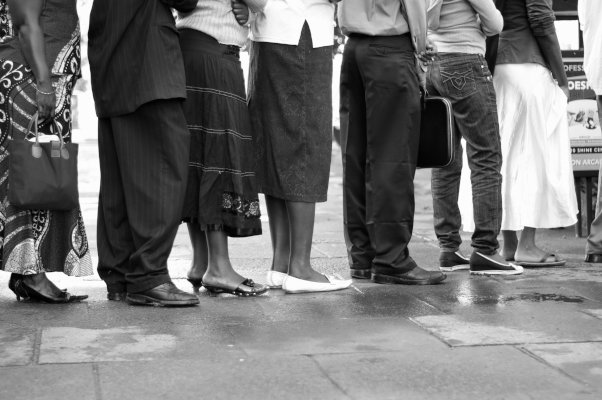
\includegraphics[height=0.35\textheight]{images/queue.jpg}}

\begin{document}

\begin{frame}
  \titlepage
\end{frame}

\section{АТД опашка}

\begin{frame}
  \frametitle{АТД: опашка}

  Хомогенна линейна структура с организация ``пръв влязъл --- пръв излязъл'' (FIFO)
  \vspace{1em}

  Операции
  \vspace{0.5em}
  \begin{itemize}
  \item \tt{create()} --- създаване на празна опашка
  \item \tt{empty()} --- проверка за празнота на опашка
  \item \tt{enqueue(x)} --- включване на елемент в края на опашката
  \item \tt{dequeue()} --- изключване на елемент от началото на опашката
  \item \tt{head()} --- достъп до първия елемент
  \end{itemize}
\end{frame}

\begin{frame}
  \frametitle{АТД: опашка}

  Свойства на операциите
  \vspace{0.5em}

  \small
  \begin{itemize}
  \item \tt{create().empty()} = \tt{true}
  \item \tt{s.enqueue(x).empty()} = \tt{false}
  \item \tt{create().head()}, \tt{create().dequeue()} --- \alert{грешка}
  \item \tt{create().enqueue(x$_1$).enqueue(x$_2$)\ldots{}enqueue(x$_n$).head() = x$_1$}
  \item \tt{create().enqueue(x$_1$).enqueue(x$_2$)\ldots{}enqueue(x$_n$).dequeue() = create().enqueue(x$_2$)\ldots{}enqueue(x$_n$)}
  \end{itemize}

\end{frame}

\begin{frame}
  \frametitle{Последователно представяне}
  \newcommand{\pha}{\phantom{$a_0$}}

  \begin{center}
    \begin{tabular}{|*{11}{c|}}
      \hline
      \rowcolor{diagramblue}
      \alt<7->{$a_{n+5}$}\pha&\pha&\alt<1>{$a_0$}\pha&$a_1$&$a_2$&\ldots&$a_n$&\alt<3->{$a_{n+1}$}\pha&\alt<4->{$a_{n+2}$}\pha&\alt<5->{$a_{n+3}$}\pha&\alt<6->{$a_{n+4}$}\pha\\
      \hline
      \rowcolor{white}
      \multicolumn 1c{\onslide<7>{\bua}}&
      \multicolumn 1c{}&
      \multicolumn 1c{\onslide<1>{\bua}}&
      \multicolumn 1c{\onslide<2->{\bua}}&
      \multicolumn 2c{}&
      \multicolumn 1c{\onslide<1-2>{\bua}}&
      \multicolumn 1c{\onslide<3>{\bua}}&
      \multicolumn 1c{\onslide<4>{\bua}}&
      \multicolumn 1c{\onslide<5>{\bua}}&
      \multicolumn 1c{\onslide<6>{\bua}}\\
      \multicolumn 1c{\onslide<7>{back}}&
      \multicolumn 1c{}&
      \multicolumn 1c{\onslide<1>{front}}&
      \multicolumn 1c{\onslide<2->{front}}&
      \multicolumn 2c{}&
      \multicolumn 1c{\onslide<1-2>{back}}&
      \multicolumn 1c{\onslide<3>{back}}&
      \multicolumn 1c{\onslide<4>{back}}&
      \multicolumn 1c{\onslide<5>{back}}&
      \multicolumn 1c{\onslide<6>{back}}
    \end{tabular}
  \end{center}

  \begin{itemize}
    \item<2-> включване на елемент (enqueue)
    \item<3-> изключване на елемент (dequeue)
  \end{itemize}
\end{frame}

\begin{frame}<1-7>
  \frametitle{Свързано представяне}

  \begin{center}
    \scriptsize
    \begin{tabular}{cccc@{}c@{}cc}
      \onslide<1-6>{\nextcell{a_0}}&\nextcell{a_1}&\nextcell{a_3}&\hspace{1ex}\ldots&$\nextarrow$&\alt<1,2>{\nilcell{a_n}}{\nextcell{a_n}}&\onslide<2->{\nilcell{a_{n+1}}}\\
      \onslide<1-6>{\bua}&\onslide<6->{\bua}&\multicolumn 3c{}&\onslide<1-3>{\bua}&\onslide<2->{\bua}\\
      \only<5-6>p\only<5>,\only<1-5>{front}&\onslide<6->{front}&\multicolumn 3c{}&\onslide<1-3>{back}&\temporal<2-3>{}p{back}
    \end{tabular}
  \end{center}

  \begin{itemize}
    \item<2-> включване на елемент (enqueue)
    \item<5-> изключване на елемент (dequeue)
  \end{itemize}
\end{frame}

\section{Задачи}

\begin{frame}
  \frametitle{Числа на Hamming}
  \newcommand{\pha}{\phantom{00}}
  \newcommand{\pho}{\phantom{0}}

  \begin{definition}
    Казваме, че $k$ е число на Hamming, ако простите делители на $k$ са сред 2, 3 и 5, т.е. $k = 2^x3^y5^z$ за $x,y,z\geq 0$.
  \end{definition}

  \textbf{Задача.} Да се изведат в нарастващ ред първите $n$ числа на Hamming.

  \pause

  \textbf{Решение:}
  \begin{center}
    \begin{tabular}{r@{\hskip 1ex}|*{11}{c|}}
      \hhline{~*{11}{-}}
      \rowcolor{diagramblue}
      \cellcolor{white}q$_2$&\alt<3-4>{\alert<4>2}\pho&\alt<4-6>{\alert<6>4}\pha&\alt<5-8>{\alert<8>6}\pha&\alt<6->8\pha&\alt<7->{10}\pha&\alt<8->{12}\pha&\pha&\pha&\pha&\pha&\pha\\
      \hhline{~*{11}{-}}
      \rowcolor{white}
      \multicolumn{12}c{}\\[0.5em]
      \hhline{~*{11}{-}}
      \rowcolor{diagramblue}
      \cellcolor{white}q$_3$&\alt<3-5>{\alert<5>3}\pho&\alt<4-8>{\alert<8>6}\pha&\alt<5->9\pha&\alt<6->{12}\pha&\alt<7->{15}\pha&\alt<8->{18}\pha&\pha&\pha&\pha&\pha&\pha\\
      \hhline{~*{11}{-}}
      \rowcolor{white}
      \multicolumn{12}c{}\\[0.5em]
      \hhline{~*{11}{-}}
      \rowcolor{diagramblue}
      \cellcolor{white}q$_5$&\alt<3-7>{\alert<7>5}\pho&\alt<4->{10}\pha&\alt<5->{15}\pha&\alt<6->{20}\pha&\alt<7->{25}\pha&\alt<8->{30}\pha&\pha&\pha&\pha&\pha&\pha\\
      \hhline{~*{11}{-}}
    \end{tabular}
    \vspace{1em}

    1%
    \onslide<5->{, 2}%
    \onslide<6->{, 3}%
    \onslide<7->{, 4}%
    \onslide<8->{, 5}%
    \onslide<9->{, 6, \ldots}
  \end{center}
\end{frame}

\begin{frame}<1-9>
  \frametitle{Минимален елемент на опашка}
  \newcommand{\pha}{\phantom{8}}
  \newcommand{\sent}{\alert s}

  \textbf{Задача.} Дадена е опашка $q$. Да се изключи от $q$ най-малкият ѝ елемент, като всички останали елементи останат в опашката (не непременно в първоначалния ред).
  \vspace{1em}
  \pause

  \textbf{Решение:}
  \begin{center}
    \begin{tabular}{|*{11}{c|}}
      \hline
      \rowcolor{diagramblue}
      \alt<4->\pha5&\alt<5->\pha3&\alt<6->\pha6&\alt<7->\pha1&\alt<8->\pha2&\alt<3-8>\sent\pha&\alt<5->5\pha&\alt<6->6\pha&\alt<7->3\pha&\alt<8->2\pha&\pha\\

      \hline
    \end{tabular}
    \vspace{1em}

    \onslide<4->{min = \temporal<5-6>531}
  \end{center}
\end{frame}

\begin{frame}
  \frametitle{Сортиране на опашки с пряка селекция}

\textbf{Задача.} Да се подредят елементите на опашка в нарастващ ред.
\vspace{1em}
\pause

\textbf{Решение:} Използваме нова опашка и прилагаме предната задача върху дадената опашка докато свърши, а минималните елементи поставяме в новата опашка.
\end{frame}

\begin{frame}
  \frametitle{Сортиране чрез сливане}

\textbf{Задача.} Да се раздели дадена опашка на две други с приблизително равна дължина.
\vspace{1em}
\pause

\textbf{Задача.} Да се слеят две опашки подредени в нарастващ ред в една.
\vspace{1em}
\pause

\textbf{Задача.} Да се сортира дадена опашка чрез сливане.
\vspace{1em}
\pause

\textbf{Решение:}
\begin{enumerate}
\item Разделяме дадената опашка на две.
\item Всяка от получените две опашки сортираме рекурсивно.
\item Сливаме двете сортирани опашки в една.
\end{enumerate}
\end{frame}

\section{STL}

\begin{frame}
  \frametitle{\tt{stl::queue<T>}}

  \begin{itemize}
  \item \tt{queue()} --- създаване на празна опашка
  \item \tt{empty()} --- проверка за празнота на опашка
  \item \tt{push(x)} --- включване на първи елемент в опашката
  \item \tt{pop()} --- изключване на последен елемент от опашката
  \item \tt{front()} --- първи елемент в опашката
  \item \tt{back()} --- последен елемент в опашката
  \item \tt{size()} --- дължина на опашката
  \item \tt{==,!=,<,>,<=,>=} --- лексикорафско сравнение на две опашки
  \end{itemize}
\end{frame}

\end{document}
